%----------------------------------------------------------------
%
%  File    :  analytical_dashboard.tex
%
%  Authors : Thomas Lerchbaumer
% 
%  Created :  19 March 2022
% 
%  Changed :  19 March
% 
%----------------------------------------------------------------

\chapter{Implementation of Averages and Grouping}
\label{chap:analytical_dashboard}
Since this paper aims to extract metrics that can contribute to an analytical dashboard this section focuses on the implementation of various groupings as well as their visualization. As the analytical dashboard is web based a short overview about its technical setup is given in section \ref{sec:tech_set}.

\section{Technical Setup}
\label{sec:tech_set}
As those implementations will contribute to an analytical dashboard the visualization of the prepared data are implemented using React. For each grouping a separate React component is created. Communication between the front- and backend is accomplished using a Rest interface. 

\begin{itemize}
\item  \verb|React|\footnote{https://react.dev/} - used for visualization
\item \verb|Python|\footnote{https://www.python.org/} - used to implement the grouping logic and interaction with the database
\item \verb|fastapi|\footnote{https://fastapi.tiangolo.com/} - Rest interface (Connection between Backend and Frontend) 
\item \verb|geopy|\footnote{https://geopy.readthedocs.io/en/stable/} - Used for calculations on latitude and longitude 
\end{itemize}
\section{Grouping Implementation}

\subsection{Grouping by Geographical Attributes}
The dataset for bus search requests (after cleaning) currently has around 230.000 entries. As the geographical calculations as well as the grouping logic are computational expensive tasks it is not feasible to redo this logic on every request. To enable real time requests with various filters onto the grouped data an additional database table is introduced. The table consists of two attributes: 
\begin{itemize}
\item \verb|parent_id (FK - search_requests(task_id)| - parent that defines a region 
\item \verb|child_id (FK - search_requests(task_id)| - entries that belong to a certain parent region  
\end{itemize}
This design comes along with several advantages. The logic for analytical requests and the grouping logic can be separated. Furthermore new entries for groupings can be added to a potential parent in a more efficient way as those entries only need to be compared to the attributes of \verb|parent_id|.

For geographical grouping the following logic is applied:
\begin{lstlisting}
radius = 20
    res = collections.defaultdict(list)
    tmp_list = collections.defaultdict(list)
    for point_a in data:
        tmp_point_a_dep = tuple((point_a['taskFrom_lng'], point_a['taskFrom_lat']))
        tmp_point_a_dest = tuple((point_a['taskTo_lng'], point_a['taskTo_lat']))
        key = point_a['id']
        found = False
        for key_b in res:
            point_b = res[key_b][0]

            tmp_point_b_dep = tuple((point_b['taskFrom_lng'], point_b['taskFrom_lat']))
            tmp_point_b_dest = tuple((point_b['taskTo_lng'], point_b['taskTo_lat']))
            actual_distance_dep = distance.great_circle(tmp_point_a_dep, tmp_point_b_dep).km
            actual_distance_dest = distance.great_circle(tmp_point_a_dest, tmp_point_b_dest).km
            if actual_distance_dep < radius and actual_distance_dest < radius:
                res[key_b].append(point_a)
                found = True
                break
        if not found:
            res[key].append(point_a)
\end{lstlisting}
This logic performs the comparison between two geographical entries. Whenever \verb|point\_b| is within a 20km radius of the departure and destination area from \verb|point\_a| \verb|point\_b| is added to the group from \verb|point\_a|. Utilizing the demonstrated database design makes it possible to still include filters like date ranges to filter groupings by date. Furthermore the averages for attributes explained in section \ref{sec:averages} can be utilized and compared to evaluate certain trends. By adjusting the logic above and removing the constraint that both destination and departure has to be within a certain range this data can further be grouped into popular destination places as well as popular departure places. Depending on the grouping technique various insights can be gathered. By analysing grouped data that mark routes (same departure/destination radius) the pricing strategy for routes with high demand can be adapted. Whereas analysing the grouping on departure places with high traffic bus operators might consider to expand their maximum approaching distance. Furthermore by changing the way how the data is fetched from the database by querying results where no bus was offered \verb|amountSearchResults == 0| a different grouping becomes available for analysing. 
\subsubsection{Visualization}
Depending on how the entries are grouped different Visualization techniques are applied. To detect departure areas with high demand a heatmap is utilized. Therefore a interactive map is utilized. Onto this map areas with high demand are plotted following a color scheme. Red circles indicate high demand whereas blue areas indicate areas with less demand as shown in figure \ref{fig:heatmap_dep}. Furthermore this visualization can be filtered by applying date ranges. Additionally areas with high demand are displayed in a table including total count of requests for a certain area, average pax as well as the average travel distance.
\newline
As a heatmap is not suitable to visualize the grouped routes those groupings are displayed using a table. Additional the table is filterable by date in order to be able to analyse the data split up into certain time periods. Furthermore the table hosts information about average pax and average travel distance. 
\begin{figure}[H]
	\centering
		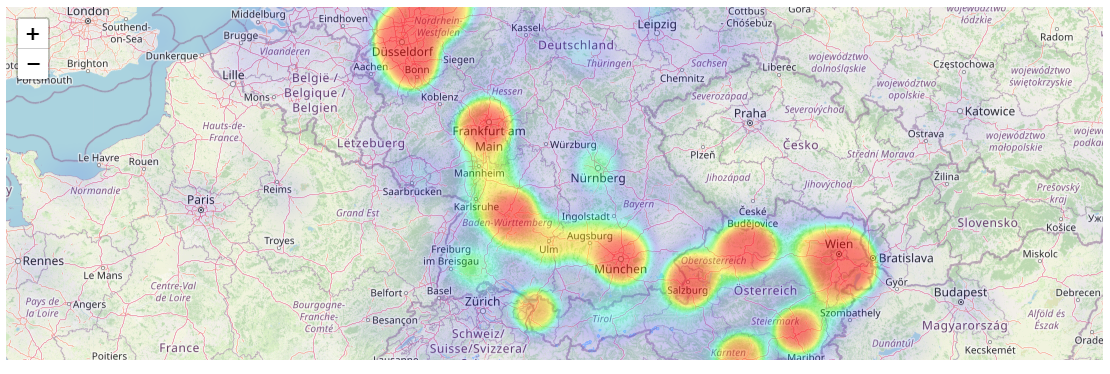
\includegraphics[width=15cm]{images/heatmap_dep}
	\caption{Interactive heatmap highlighting departure places with high demand - [source:[author]]}
	\label{fig:heatmap_dep}
\end{figure}


\subsection{Grouping by Time}
In contrast to geographical grouping, groupings by time do not require a table within the database in order to process requests in real time. To group requests by time the following logic is applied to the fetched data: 
\begin{lstlisting}
def group_requests_by_time(data):
    df = pd.DataFrame(data)
    df = pd.to_datetime(df[0])
    grouped = df.groupby(df.dt.hour).count()
    for name in grouped.index:
        tmp = {"x": str(name) + ":00", "y": int(grouped.loc[name])}
        res[0]['data'].append(tmp)
    return res
\end{lstlisting}
To group search requests by days the following logic is applied: 
\begin{lstlisting}
def group_requests_by_day(data):
    data_format = pd.DataFrame(data)
    data_format = pd.to_datetime(data_format[0], format='%Y-%m-%d %H:%M:%S')
    grouped = data_format.groupby([data_format.dt.year, data_format.dt.month, data_format.dt.day]).count()
    res = []
    for name in grouped.index:
        date = str(name[0]) + "-" + str(name[1]) + "-" + str(name[2])
        tmp = {"value": int(grouped.loc[name]), "day": date}
        res.append(tmp)
    res = sorted(res, key=lambda x: x['day'])
    return res
\end{lstlisting}
Depending on which attribute e.g. \verb|createdAt| \verb|taskFrom_time| are fetched from the database different groupings become available. Both attributes provide valuable information. When the data is grouped by utilizing the attribute \verb|createdAt| the success rate of previous marketing campaigns can be evaluated. Furthermore this information can be consulted to plan future marketing campaigns. By grouping the data using the attribute \verb|taskFrom_time| seasonal patterns become visible as shown in \ref{fig:dep_grouping}
\subsubsection{Visualization}
The hourly groupings are visualized using a line chart as demonstrated in figure \ref{fig:hourly_grouping}.
\begin{figure}[H]
	\centering
		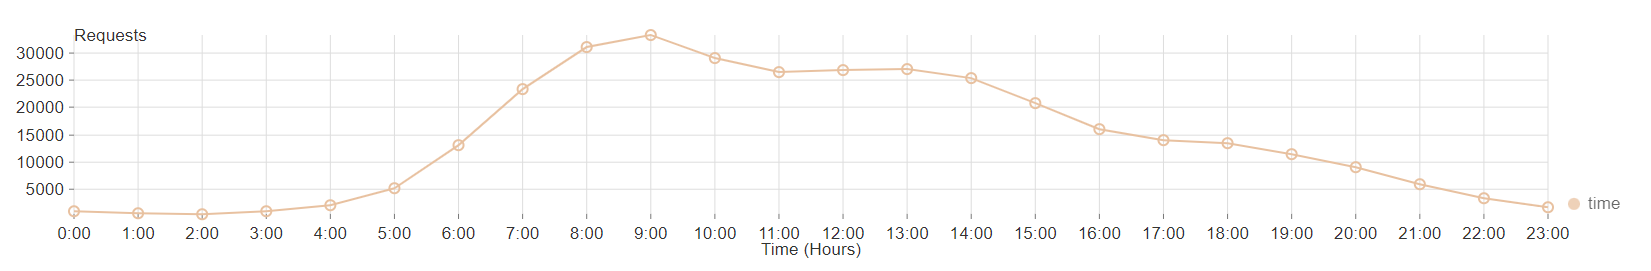
\includegraphics[width=15cm]{images/requests_hour}
	\caption{***PLACEHOLDER Requests grouped on hourly basis- [source:[author]]}
	\label{fig:hourly_grouping}
\end{figure}
By analysing figure \ref{fig:hourly_grouping} the highest the most search requests are made at around 9am. By hovering over each data point the amount of search requests become visible. 
\newline
 
\begin{figure}[H]
	\centering
		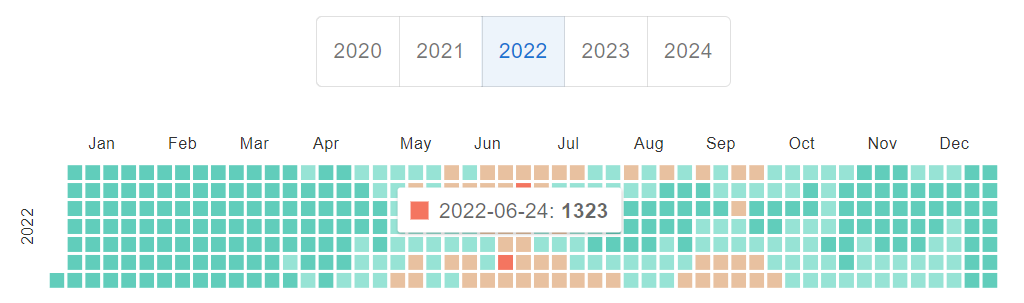
\includegraphics[width=15cm]{images/grouping_by_taskFrom}
	\caption{ **PLACEHOLDER Daily grouping of Departure Dates- [source:[author]]}
	\label{fig:grouping_dep_daily}
\end{figure}
The grouping by day is visualized by an heatmap mapped to an calendar. By investigating the results for different years seasonal patterns become visible.
\begin{figure}[H]
	\centering
		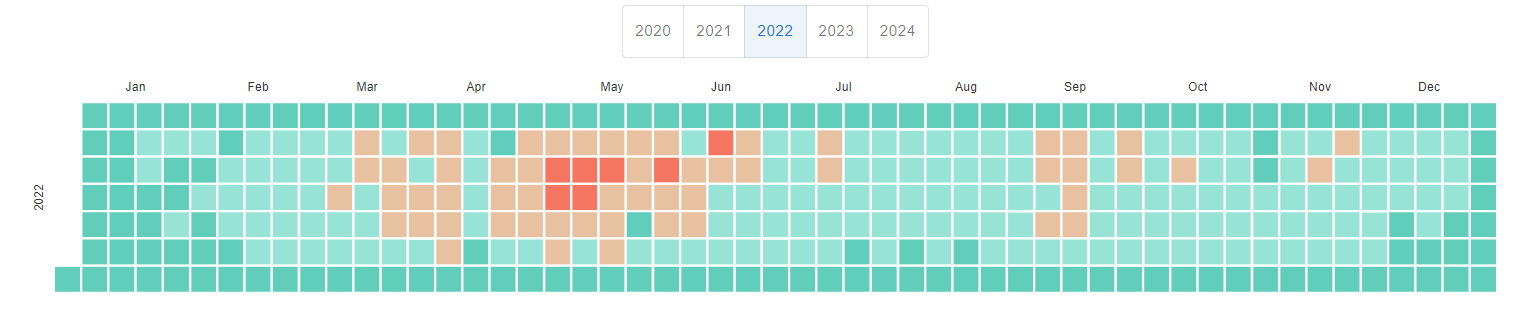
\includegraphics[width=15cm]{images/grouping_by_created_at}
	\caption{**PLACEHOLDER Daily grouping of when search requests are made- [source:[author]]}
	\label{fig:grouping_search_daily}
\end{figure}
All of the extracted groupings are filterable by date ranges in real time. Furthermore whenever a filter is applied the average pax as well as the average distance is provided to the user.